\documentclass[12pt]{beamer}
\usepackage{amsmath,amssymb,amsfonts,amsthm}
\beamertemplatefootpagenumber
\usepackage{threeparttable}
\geometry{paperwidth=150mm,paperheight=125mm}
\usepackage{lipsum}
\usepackage{ragged2e} % 文字向兩邊對齊
\useinnertheme{rectangles}  % change the theme

\usepackage{float}
\usepackage{multirow}
\usepackage{makecell}
\usepackage{siunitx}
\usepackage{csvsimple}
\usepackage{tikz}
%\usepackage{booktabs}

%打中文需要以下packages
\usepackage{xeCJK} 
\setCJKmainfont[BoldFont={cwTeXHeiBold}, ItalicFont={FandolSong}]{cwTeXMing} %Overleaf 中文字型設定
%\setCJKmainfont[BoldFont={cwTeX Q HeiZH}, ItalicFont={新細明體}]{cwTeX Q Ming}	
\XeTeXlinebreaklocale "zh"
\XeTeXlinebreakskip = 0pt plus 1pt %這兩行一定要加,中文才能自動換行

\usepackage{listings}
\usepackage{array}
\usepackage{xcolor}
\usepackage{colortbl}
\usepackage{collcell}
\usepackage{mathtools}

% %%% Parameters
% % Constants
% \newcommand\maxval{120}
% \newcommand\baseval{10}
% \newcommand\minval{5}
% \newcommand\gradsteps{1}

% % Colours
% \colorlet{tabbase}{green!50}
% \colorlet{tabmax}{red!!black!50}
% \colorlet{tabmin}{blue!!cyan!30}

% % Colour series
% \definecolorseries{lower}{rgb}{last}{tabmin}{tabbase}
% \definecolorseries{higher}{rgb}{last}{tabbase}{tabmax}
% \resetcolorseries[\gradsteps]{lower}
% \resetcolorseries[\gradsteps]{higher}

% % The auxiliary commands to colourise cells
% \NewDocumentCommand\vcellcolor{m}{%
%   \centering
%   \ifdim#1pt=\baseval pt\cellcolor{tabbase}%
%   \else%
%     \ifdim#1pt>\baseval pt%
%       \ifdim#1pt>\maxval pt\cellcolor{tabmax}%
%       \else%
%         \cellcolor{higher!![\fpeval{floor(\gradsteps*(#1-\baseval)/(\maxval-\baseval))}]}
%       \fi%
%     \else%
%       \ifdim#1pt<\minval pt\cellcolor{lower!![0]}
%       \else%
%         \cellcolor{lower!![\fpeval{ceil(\gradsteps*(#1-\minval)/(\baseval-\minval))}]}
%       \fi%
%     \fi%
%   \fi #1}
% \newcolumntype{C}[1]{%
%   >{\collectcell\vcellcolor}wc{#1}<{\endcollectcell}}


\title[]  
{Demand System Estimation}
\subtitle[short subtitle]{Group 5}

\author{黎宏濬 \ 林孝儒 \ 張立宏 \ 許震浩}
\institute[short]{\inst{}Department of Agricultural Economics, NTU}

\date
 {October 18, 2024}
 
\AtBeginSection[]{
    % \begin{frame}[plain]  % plain 选项去除页眉页脚
    %     \vfill
    %     \figureing
    %     \usebeamerfont{section title}\insertsectionhead\par
    %     \vfill
    % \end{frame}
    \begin{frame}
        \frametitle{Outline}
        % Display the entire table of contents instead of limiting to 1-\thesection
        \tableofcontents[currentsection]
    \end{frame}
} 

\begin{document}

% Title page
\begin{frame}{}
    \titlepage
\end{frame}

% Table of Contents slide
\begin{frame}
    \frametitle{Outline}
    \tableofcontents[]
\end{frame}

\begin{frame}{產品定義}
	\begin{figure}
		\centering
		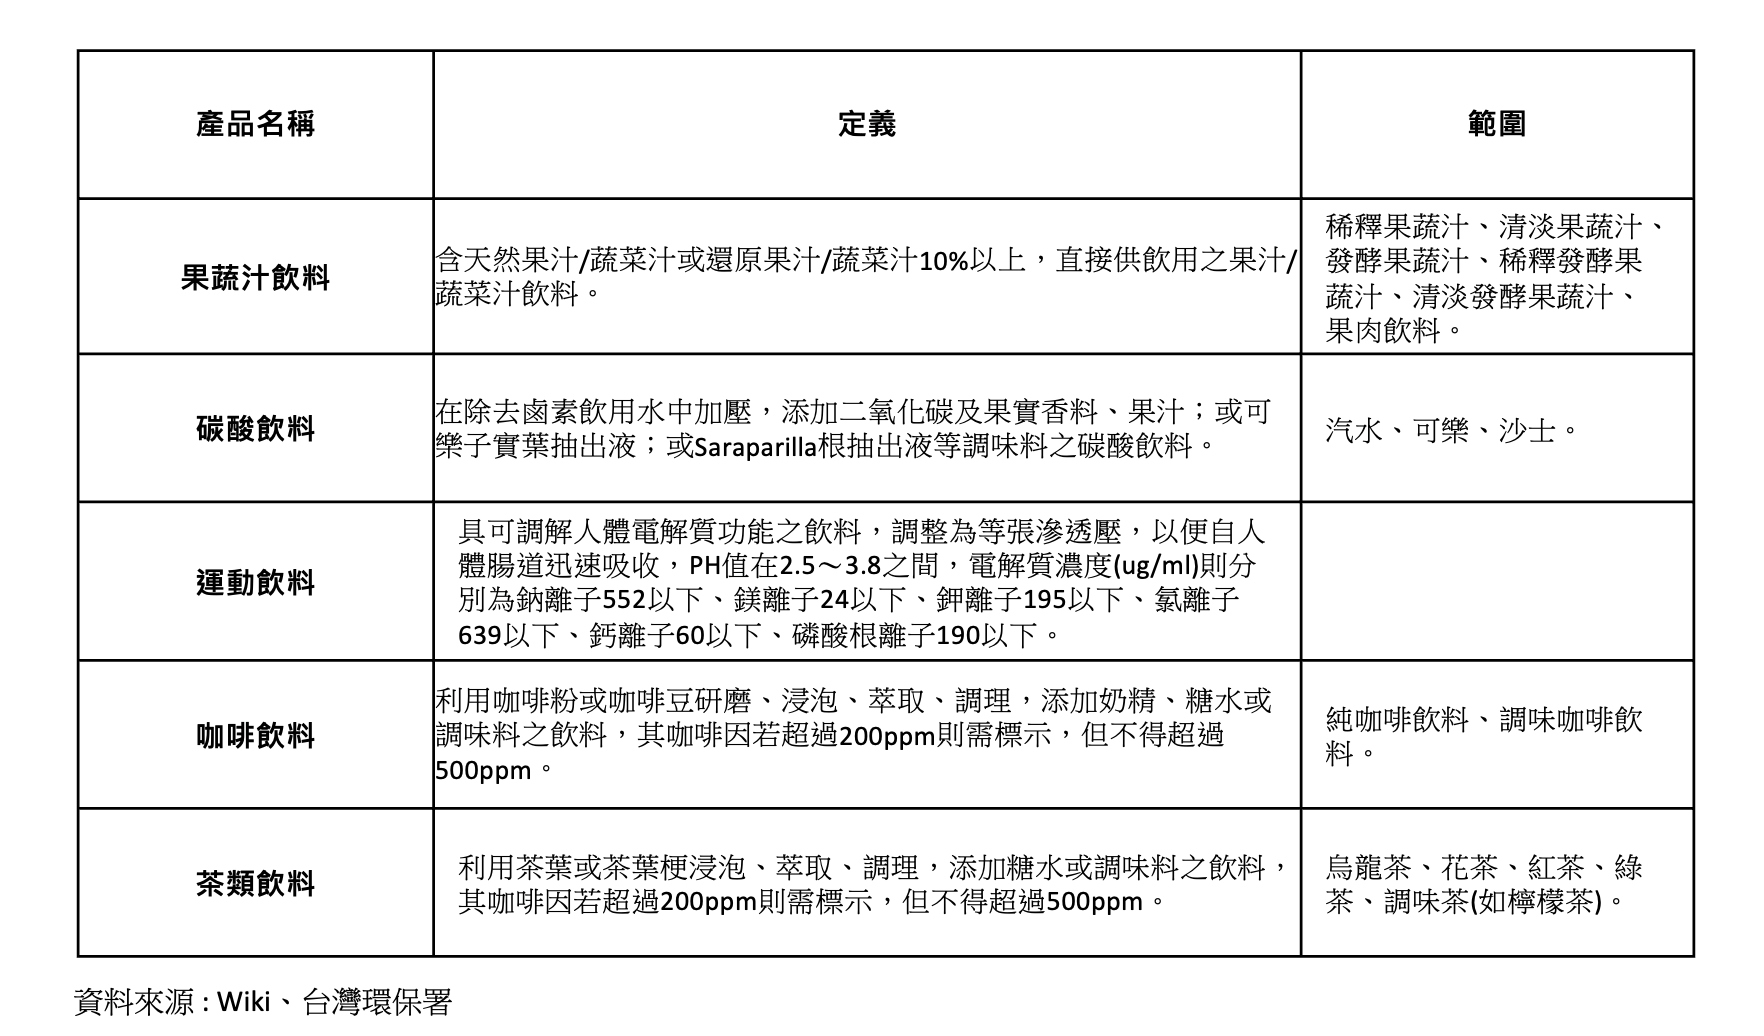
\includegraphics[width=1\textwidth]{figures/產品定義.png}
		\caption{資料期間: 1991 - 2023}
	\end{figure}
\end{frame}

\section{資料整理過程}

\begin{frame}{資料整理重點過程}
	\begin{itemize}
		\item 年份和月份提取:利用 gsub 函數去掉「年」和「月」字,並將年份和月份轉換為數值型
		\item 年份轉換:將民國年轉換為西元年,並將所有收入數據轉換為數值型格式(去掉逗號)
		\item 缺失值填補:利用 nafill 函數按順序填補年份和月份的缺失值
		\item 重新命名:將產品名稱(果蔬汁、碳酸飲料等)及其對應的數據欄位分別改為英文名稱  
		\item 將銷售數據、物價數據、薪資數據進行 full join, 也就是透過相同的年份和月份進行合併
	\end{itemize}
\end{frame}

\section{分析結果}


\begin{frame}{AIDS}
\[
	w_i = \alpha_i + \sum_{j=1}^{5} \gamma_{ij} \ln(P_j) + \beta_i \ln\left(\frac{X}{P}\right),
\]
\begin{itemize}
	\item $w_i = \frac{P_i Q_i}{X}$: expenditure share of the $i$-th beverage category
	\begin{itemize}
		\item $P_i$ is the price of the $i$-th beverage
		\item $Q_i$ is the quantity of the $i$-th beverage
		\item $X$ is the total expenditure on all beverages, which may vary with monthly income
	\end{itemize}
	\item $\ln(P_j)$: The natural logarithm of the price of the $j$-th beverage
	\item $P$: Price index, typically approximated by the Stone price index:
	\begin{equation*}
	\ln(P) = \sum_{j=1}^{5} w_j \ln(P_j),
	\end{equation*}
	where $w_j$ is the expenditure share of the $j$-th beverage
	\item $\alpha_i$, $\gamma_{ij}$, $\beta_i$: Parameters to be estimated for each beverage category
\end{itemize}
\end{frame}


\begin{frame}{估計結果}
    \begin{table}[h]
    \centering
    \footnotesize{
    \begin{tabular}{lccccc}
        \hline & 果蔬汁飲料 & 碳酸飲料 & 運動飲料 & 咖啡飲料 & 茶類飲料 \\
		\hline 
		& \phantom{3}1.164$^{***}$ & \phantom{3}0.417$^{***}$ & \phantom{3}-0.268$^{***}$ & \phantom{3}0.759$^{***}$ & \phantom{3}-1.072$^{***}$ \\[-2ex]
		\raisebox{2ex}{$\alpha$} & (0.079) & (0.116) & (0.023) & (0.056) & (0.192) \\[0ex]
		& \phantom{3}-0.085$^{***}$ & -0.017 & \phantom{3}0.028$^{***}$ & \phantom{3}-0.065$^{***}$ & \phantom{3}0.139$^{***}$ \\[-2ex]
		\raisebox{2ex}{$\beta$} & (0.007) & (0.009) & (0.005) & (0.005) & (0.016) \\[0ex]
		\hline
		$R^2$ & 0.439 & 0.284 & 0.152 & 0.684 & 0.241 \\
        \hline
    \end{tabular}}
    \caption{Coefficients and R-squared values of expenditure shares}
    % \label{turns1}    
    \end{table}

	$\alpha$(截距項): 代表了每個飲料類別的消費支出份額的常數部分,反映了不同飲料類別的基礎需求水準
	\begin{itemize}
		\item 果蔬汁的alpha參數最大,說明果蔬汁在所有飲料中具有最高的基本需求
		\item 茶類飲料的alpha參數最小,說明茶類飲料在所有飲料中的基本需求最低
	\end{itemize}

	$\beta$: 衡量了支出變動對每個飲料類別的需求影響,beta參數越大,飲料需求對支出的變化反應越強
	\begin{itemize}
		\item 果蔬汁的beta參數最小,表示隨著總支出增加,消費者對果蔬汁的需求會顯著減少
		\item 茶類飲料的beta參數最大,支出增加對茶類飲料需求有顯著的正向影響
	\end{itemize}
\end{frame}

\begin{frame}{估計結果}
	\begin{table}[h]
		\begin{center} \footnotesize{
		\begin{tabular}{lccccc}
			\hline
			 & 果蔬汁飲料 & 碳酸飲料 & 運動飲料 & 咖啡飲料 & 茶類飲料 \\
			\hline
			& \phantom{3}0.082$^{***}$ & \phantom{3}-0.111$^{***}$ & \phantom{1}-0.015$^{*}$ & \phantom{1}0.030$^{*}$ & 0.015 \\[-1.5ex]
			\raisebox{2ex}{$\gamma_{\text{果蔬汁}}$} & (0.018) & (0.016) & (0.006) & (0.013) & (0.017) \\[0ex]
			& \phantom{3}-0.112$^{***}$ & \phantom{3}-0.118$^{***}$ & \phantom{3}-0.060$^{***}$ & 0.016 & \phantom{3}0.274$^{***}$ \\[-2ex]
			\raisebox{2ex}{$\gamma_{\text{碳酸}}$} & (0.016) & (0.027) & (0.008) & (0.017) & (0.023) \\[0ex]
			& \phantom{1}-0.015$^{*}$ & \phantom{3}-0.060$^{***}$ & \phantom{3}-0.037$^{***}$ & \phantom{3}0.379$^{***}$ & \phantom{3}0.073$^{***}$ \\[-2ex]
			\raisebox{2ex}{$\gamma_{\text{運動}}$} & (0.006) & (0.008) & (0.004) & (0.005) & (0.011) \\[0ex]
			& \phantom{1}0.030$^{*}$ & 0.016 & \phantom{3}0.039$^{***}$ & \phantom{3}0.170$^{***}$ & \phantom{3}0.257$^{***}$ \\[-2ex]
			\raisebox{2ex}{$\gamma_{\text{咖啡}}$} & (0.013) & (0.017) & (0.005) & (0.018) & (0.012) \\[0ex]
			& 0.150 & \phantom{3}0.274$^{***}$  & \phantom{3}0.074$^{***}$ & \phantom{3}0.257$^{***}$ & \phantom{2}-0.105$^{**}$\\[-2ex]
			\raisebox{2ex}{$\gamma_{\text{茶類}}$} & (0.017) & (0.023) & (0.011) & (0.012) & (0.036) \\[0ex]
			\hline
			$R^2$ & 0.428 & 0.493 & 0.605 & 0.685 & 0.759 \\
			\hline
		\end{tabular} }
		\end{center}
		\caption{\footnotesize Coefficients and R-squared values of quantities}
		\label{turns2}
	\end{table}

\end{frame}

\begin{frame}{Adding-up check}
	Adding-up 要求$\alpha$加總應該為 1
	\[
		\sum_i \alpha_i = 1.164+0.417 -0.268+ 0.759-1.072 = 1
	\]
	符合 Adding-up 條件
	% \begin{figure}
	% 	\centering
	% 	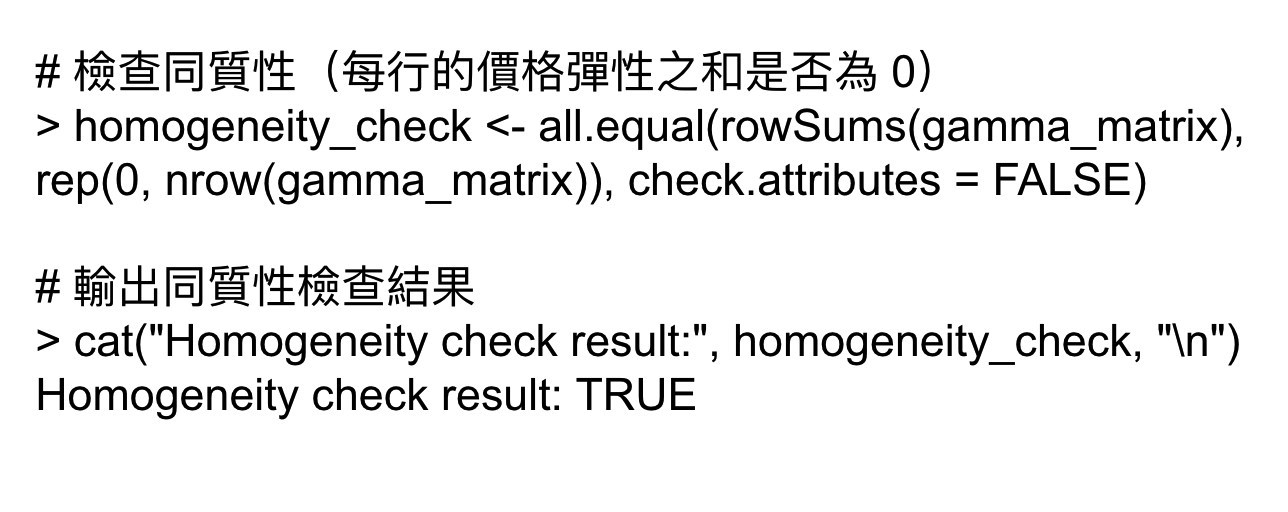
\includegraphics[width=0.7\textwidth]{figures/homogeneity.png}
	% 	\caption{Homogeneity check}
	% \end{figure}
\end{frame}

\begin{frame}{Homogeneity check}
	Homogeneity 要求 $\gamma$ 行列加總應該為 0
	\[
		\sum_i \gamma_{ij} = 0 \quad \forall j
	\]
	\[
		\sum_j \gamma_{ij} = 0 \quad \forall i
	\]
	\begin{figure}
		\centering
		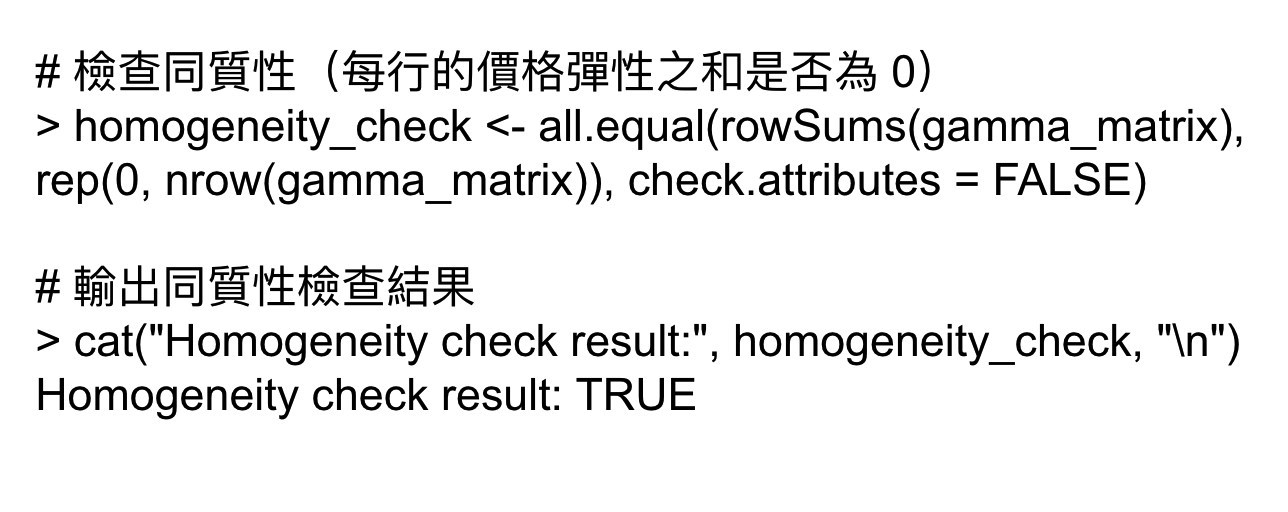
\includegraphics[width=0.7\textwidth]{figures/homogeneity.png}
		\caption{Homogeneity check}
	\end{figure}
\end{frame}

\begin{frame}{Symmetry check}
	Symmetry 要求產品交叉價格應該對稱,因為商品 $i$ 對 商品$j$ 的影響應該等於商品 $j$ 對 商品$i$ 的影響
	\[
		\gamma_{ij} = \gamma_{ji} \quad \forall i \neq j
	\]
	\begin{figure}
		\centering
		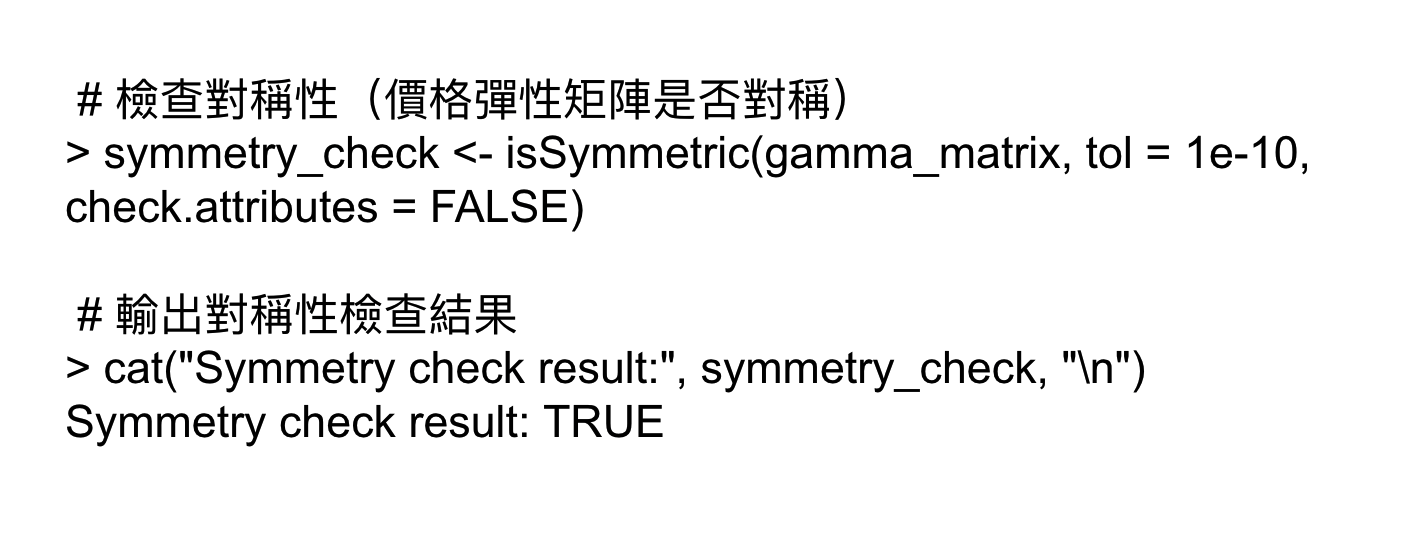
\includegraphics[width=0.7\textwidth]{figures/symmetry.png}
		\caption{Summetry check}
	\end{figure}
\end{frame}

% \begin{frame}{檢查同質性}
% \textbf{R 代碼:}

% \begin{verbatim}
% # 檢查同質性(每行的價格彈性之和是否為 0)
% homogeneity_check <- all.equal(rowSums(gamma_matrix), 
%                                rep(0, nrow(gamma_matrix)), 
%                                check.attributes = FALSE)
% # 輸出同質性檢查結果
% cat("Homogeneity check result:", homogeneity_check, "\n")
% \end{verbatim}

% \textbf{輸出結果:}
% \texttt{Homogeneity check result: TRUE}
% \end{frame}

% \begin{frame}{檢查對稱性}
% \textbf{R 代碼:}

% \begin{verbatim}
% # 檢查同質性(每行的價格彈性之和是否為 0)
% homogeneity_check <- all.equal(rowSums(gamma_matrix), 
%                                rep(0, nrow(gamma_matrix)), 
%                                check.attributes = FALSE)
% # 輸出同質性檢查結果
% cat("Homogeneity check result:", homogeneity_check, "\n")
% \end{verbatim}

% \textbf{輸出結果:}
% \texttt{Homogeneity check result: TRUE}
% \end{frame}

\begin{frame}{支出彈性 (Expenditure Elasticity)}
	\textbf{支出彈性 (Expenditure Elasticity)}
	\[
		\varepsilon_i^x = 1 + \frac{\beta_i}{w_i}
	\]
	\begin{itemize}
		\item 若 \( \varepsilon_i^x > 1 \),則商品 \( i \) 為奢侈品;
		\item 若 \( \varepsilon_i^x < 1 \),則商品 \( i \) 為必需品。
	\end{itemize}
\end{frame}

\begin{frame}{支出彈性 (Expenditure Elasticity)}
	\begin{table}[tbh]
		\begin{tabular}{c rrrrr}
			\noalign{\hrule height 0.8pt}
		% 	\(\xmathstrut[1]{1}\)%
			 & 果蔬汁 & 碳酸 & 運動 & 咖啡 & 茶 \\
			\noalign{\hrule height 0.5pt}
			% \(\xmathstrut[0]{0.25}\)%
			支出彈性 &  0.548  & 0.908 & 1.376 & 0.485 & 1.321 \\
			\noalign{\hrule height 0.8pt}
		\end{tabular}
	\end{table}
	\begin{itemize}
		\item 果蔬汁飲料、碳酸飲料、茶類飲料為必需品
		\item 茶類飲料與運動飲料為奢侈品
	\end{itemize}
\end{frame}

\begin{frame}{自價格彈性 (Own-price Elasticity) / 交叉價格彈性 (Cross-price Elasticity)}
	\textbf{自價格彈性 (Own-price Elasticity)}
	\[
	\varepsilon_{ii} = -1 + \frac{\gamma_{ii}}{w_i} - \beta_i \log \left( \frac{x}{P} \right)
	\]
	\textbf{交叉價格彈性 (Cross-price Elasticity)}
	\[
	\varepsilon_{ij} = \frac{\gamma_{ij}}{w_i} - \beta_i \log \left( \frac{x}{P} \right)
	\]
	\begin{itemize}
		\item 如果 \( \varepsilon_{ij} > 0 \),商品 \( i \) 和 \( j \) 為替代品;
		\item 如果 \( \varepsilon_{ij} < 0 \),商品 \( i \) 和 \( j \) 為互補品。
	\end{itemize}
\end{frame}

\begin{frame}{自價格彈性 (Own-price Elasticity) / 交叉價格彈性 (Cross-price Elasticity)}
	\begin{table}[tbh]
		% \renewcommand\arraystretch{1.1}
		% \centering
		\begin{tabular}{c rrrrr}
			\noalign{\hrule height 0.8pt}
		% 	\(\xmathstrut[1]{1}\)%
			 & 果蔬汁 & 碳酸 & 運動 & 咖啡 & 茶 \\
			\noalign{\hrule height 0.5pt}
			% \(\xmathstrut[0]{0.25}\)%
			果蔬汁 & -0.482 & -0.516 & -0.049 & 0.223 & 0.275 \\
			碳酸 &-0.605 & -1.645 & -0.329 & 0.106 & 1.565 \\
			運動 &  -0.278 & -0.882 & -1.531 & 0.480 & 0.835 \\
			咖啡 & 0.340  & 0.225  & 0.346  & 0.407 & -1.803 \\
			% \(\xmathstrut[0.25]{0}\)%
			茶 & -0.025 & 0.576  & 0.147  & -0.635 & -1.383 \\
			\noalign{\hrule height 0.8pt}
		\end{tabular}
	\end{table}
	飲料類別間的價格交叉彈性和自身價格彈性,說明某一飲料類別的價格變化如何影響另一類別或自身的需求
	\begin{itemize}
		\item 果蔬汁與碳酸飲料可能是互補品
		\item 碳酸飲料與運動飲料可能是互補品,與茶類飲料可能是替代品
		\item 運動飲料與咖啡飲料和茶類飲料可能是替代品
		\item 咖啡飲料與茶類飲料可能是互補品
		\item 碳酸飲料的自身價格彈性絕對值最大,需求量受定價的變化最大
	\end{itemize}
\end{frame}

\begin{frame}{ADF Test Results}
	\textbf{ADF 單根檢定的目的是什麼?} \\
	\begin{itemize}
	\item ADF 檢定的主要目的是判斷時間序列數據是否為平穩時間序列。平穩時間序列的統計特徵(如平均數和變異數)在整個時間區段內保持穩定,這對於許多時間序列分析方法來說是必要條件。如果時間序列是非平穩的,通常需要對其進行差分處理(如一階差分)來轉換為平穩序列。
	\item 檢定統計量(Test Statistic):這是 ADF 檢驗的主要結果,用來判斷時間序列是否具有單根(非平穩)。
	\item 臨界值(Critical Value),用來判斷檢驗統計量是否顯著。當檢定統計量小於這些臨界值時,表示可以拒絕單根假設,即時間序列是平穩的。
	\end{itemize}
\end{frame}

\begin{frame}{ADF Test Results}
	\begin{table}[htbp]
	\centering
		\begin{tabular}{lcccc}
		\hline
		\textbf{Variable} & \makecell{\textbf{Test} \\ \textbf{Statistic}} & \makecell{\textbf{Critical} \\ \textbf{Value 1\%}} & \makecell{\textbf{Critical} \\ \textbf{Value 5\%}} & \makecell{\textbf{Critical} \\ \textbf{Value 10\%}} \\
		\hline
		果蔬汁價格 & -6.172 & -3.44 & -2.87 & -2.57 \\
		碳酸飲料價格  & -5.116 & -3.44 & -2.87 & -2.57 \\
		運動飲料價格        & -3.707 & -3.44 & -2.87 & -2.57 \\
		咖啡飲料價格        & -3.930 & -3.44 & -2.87 & -2.57 \\
		茶類飲料價格            & -3.069 & -3.44 & -2.87 & -2.57 \\
		\hline
		\end{tabular}
		\caption{單根檢定結果: 每種飲料的價格變量的 ADF 檢定統計量在5\%水準下皆小於臨界值拒絕單根假設,因此飲料的價格變量是平穩的。}
	\end{table}
\end{frame}

\begin{frame}{Durbin-Watson test}
	\begin{itemize}
		\item FruitVegetableJuice\_price
		\begin{itemize}
			\item $DW =  0.31032$
		\end{itemize}
		\item CarbonatedBeverage\_price 
		\begin{itemize}
			\item $DW = 0.40014$
		\end{itemize}
		\item SportsDrink\_price 
		\begin{itemize}
			\item $DW = 0.3316$
		\end{itemize}
		\item CoffeeDrink\_price 
		\begin{itemize}
			\item $DW = 0.45798$
		\end{itemize}
		\item TeaDrink\_price 
		\begin{itemize}
			\item $DW = 0.22287$
		\end{itemize}
	\end{itemize} 
\end{frame}

\end{document}
